\section{BusyBox}

\begin{frame}
  \frametitle{Why BusyBox?}
  \begin{itemize}
  \item A Linux system needs a basic set of programs to work
    \begin{itemize}
    \item An init program
    \item A shell
    \item Various basic utilities for file manipulation and system
      configuration
    \end{itemize}
  \item In normal GNU/Linux systems, these programs are provided by
    different projects
    \begin{itemize}
    \item \code{coreutils}, \code{bash}, \code{grep}, \code{sed},
      \code{tar}, \code{wget}, \code{modutils}, etc. are all different
      projects
    \item A lot of different components to integrate
    \item Components not designed with embedded systems constraints in
      mind: they are not very configurable and have a wide range of
      features
    \end{itemize}
  \item BusyBox is an alternative solution, extremely common on
    embedded systems
  \end{itemize}
\end{frame}

\begin{frame}
  \frametitle{General purpose toolbox: BusyBox}
  \begin{columns}
    \column{0.75\textwidth}
      \url{https://www.busybox.net/}
      \begin{itemize}
      \item Rewrite of many useful UNIX command line utilities
        \begin{itemize}
        \item Created in 1995 to implement a rescue and installer
         system for Debian, fitting in a single floppy disk (1.44 MB)
        \item Integrated into a single project, which makes it easy to
          work with
        \item Great for embedded systems: highly configurable,
          no unnecessary features
        \item Called the {\em Swiss Army Knife of Embedded Linux}
        \end{itemize}
      \item License: GNU GPLv2
      \item Alternative: Toybox, BSD licensed (\url{https://en.wikipedia.org/wiki/Toybox})
      \end{itemize}
    \column{0.25\textwidth}
    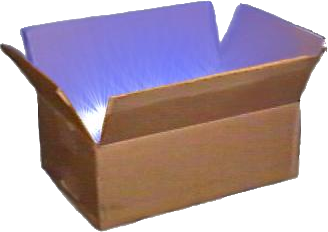
\includegraphics[width=\textwidth]{common/busybox.png}
  \end{columns}
\end{frame}

\begin{frame}
  \frametitle{BusyBox in the root filesystem}
  \begin{columns}
    \column{0.65\textwidth}
      \begin{itemize}
      \item All the utilities are compiled into a single executable,
        \code{/bin/busybox}
        \begin{itemize}
        \item Symbolic links to \code{/bin/busybox} are created for each
          application integrated into BusyBox
        \end{itemize}
      \item For a fairly featureful configuration, less than 500 KB
        (statically compiled with uClibc) or less than 1 MB (statically
        compiled with glibc).
      \end{itemize}
    \column{0.35\textwidth}
      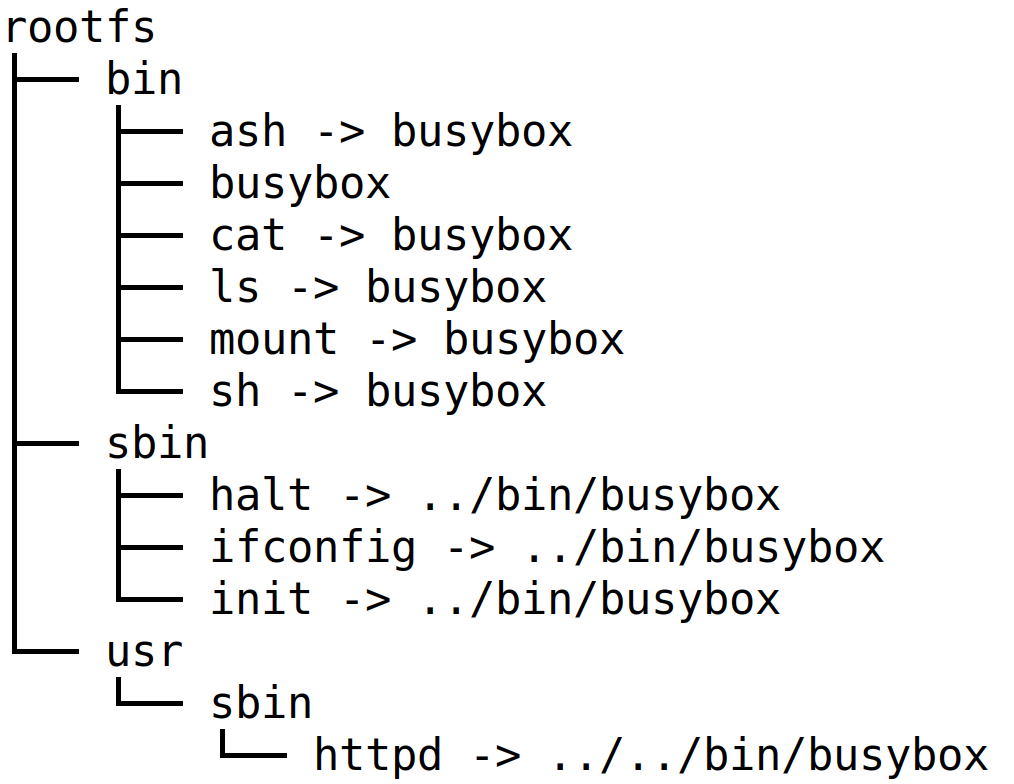
\includegraphics[width=\textwidth]{slides/sysdev-busybox/busybox-tree.png}
  \end{columns}
\end{frame}

\begin{frame}[fragile]
  \frametitle{BusyBox - Most commands in one binary}
  \tiny
  % To update this list, compile busybox with "make allyesconfig" on x86
  % Then run "./busybox" and reduce the terminal width until the first
  % line ends with "blkid". Then copy the output here.
  \begin{verbatim}
[, [[, acpid, add-shell, addgroup, adduser, adjtimex, arch, arp, arping, ash, awk, base64, basename, bc, beep, blkdiscard, blkid,
blockdev, bootchartd, brctl, bunzip2, bzcat, bzip2, cal, cat, chat, chattr, chgrp, chmod, chown, chpasswd, chpst, chroot, chrt,
chvt, cksum, clear, cmp, comm, conspy, cp, cpio, crond, crontab, cryptpw, cttyhack, cut, date, dc, dd, deallocvt, delgroup,
deluser, depmod, devmem, df, dhcprelay, diff, dirname, dmesg, dnsd, dnsdomainname, dos2unix, dpkg, dpkg-deb, du, dumpkmap,
dumpleases, echo, ed, egrep, eject, env, envdir, envuidgid, ether-wake, expand, expr, factor, fakeidentd, fallocate, false,
fatattr, fbset, fbsplash, fdflush, fdformat, fdisk, fgconsole, fgrep, find, findfs, flock, fold, free, freeramdisk, fsck,
fsck.minix, fsfreeze, fstrim, fsync, ftpd, ftpget, ftpput, fuser, getopt, getty, grep, groups, gunzip, gzip, halt, hd, hdparm,
head, hexdump, hexedit, hostid, hostname, httpd, hush, hwclock, i2cdetect, i2cdump, i2cget, i2cset, i2ctransfer, id, ifconfig,
ifdown, ifenslave, ifplugd, ifup, inetd, init, insmod, install, ionice, iostat, ip, ipaddr, ipcalc, ipcrm, ipcs, iplink, ipneigh,
iproute, iprule, iptunnel, kbd_mode, kill, killall, killall5, klogd, last, less, link, linux32, linux64, linuxrc, ln, loadfont,
loadkmap, logger, login, logname, logread, losetup, lpd, lpq, lpr, ls, lsattr, lsmod, lsof, lspci, lsscsi, lsusb, lzcat, lzma,
lzop, makedevs, makemime, man, md5sum, mdev, mesg, microcom, mim, mkdir, mkdosfs, mke2fs, mkfifo, mkfs.ext2, mkfs.minix, mkfs.vfat,
mknod, mkpasswd, mkswap, mktemp, modinfo, modprobe, more, mount, mountpoint, mpstat, mt, mv, nameif, nanddump, nandwrite,
nbd-client, nc, netstat, nice, nl, nmeter, nohup, nologin, nproc, nsenter, nslookup, ntpd, nuke, od, openvt, partprobe, passwd,
paste, patch, pgrep, pidof, ping, ping6, pipe_progress, pivot_root, pkill, pmap, popmaildir, poweroff, powertop, printenv, printf,
ps, pscan, pstree, pwd, pwdx, raidautorun, rdate, rdev, readahead, readlink, readprofile, realpath, reboot, reformime,
remove-shell, renice, reset, resize, resume, rev, rm, rmdir, rmmod, route, rpm, rpm2cpio, rtcwake, run-init, run-parts, runlevel,
runsv, runsvdir, rx, script, scriptreplay, sed, sendmail, seq, setarch, setconsole, setfattr, setfont, setkeycodes, setlogcons,
setpriv, setserial, setsid, setuidgid, sh, sha1sum, sha256sum, sha3sum, sha512sum, showkey, shred, shuf, slattach, sleep, smemcap,
softlimit, sort, split, ssl_client, start-stop-daemon, stat, strings, stty, su, sulogin, sum, sv, svc, svlogd, svok, swapoff,
swapon, switch_root, sync, sysctl, syslogd, tac, tail, tar, taskset, tc, tcpsvd, tee, telnet, telnetd, test, tftp, tftpd, time,
timeout, top, touch, tr, traceroute, traceroute6, true, truncate, ts, tty, ttysize, tunctl, ubiattach, ubidetach, ubimkvol,
ubirename, ubirmvol, ubirsvol, ubiupdatevol, udhcpc, udhcpc6, udhcpd, udpsvd, uevent, umount, uname, unexpand, uniq, unix2dos,
unlink, unlzma, unshare, unxz, unzip, uptime, users, usleep, uudecode, uuencode, vconfig, vi, vlock, volname, w, wall, watch,
watchdog, wc, wget, which, who, whoami, whois, xargs, xxd, xz, xzcat, yes, zcat, zcip
  \end{verbatim}
  \vfill
  \footnotesize
  Source: run \code{/bin/busybox} - July 2021 status
\end{frame}

\begin{frame}
  \frametitle{Configuring BusyBox}
  \begin{itemize}
  \item Get the latest stable sources from \url{https://busybox.net}
  \item Configure BusyBox (creates a \code{.config} file):
    \begin{itemize}
    \item \code{make defconfig}\\
      Good to begin with BusyBox.\\
      Configures BusyBox with all options for regular users.
    \item \code{make allnoconfig}\\
      Unselects all options. Good to configure only what you need.
    \end{itemize}
  \item \code{make menuconfig} (text)\\
    Same configuration interfaces as the ones used by the Linux kernel
    (though older versions are used, causing \code{make xconfig} to
    be broken in recent distros).
  \end{itemize}
\end{frame}

\begin{frame}
  \frametitle{BusyBox make menuconfig}
  \begin{columns}
    \column{0.5\textwidth}
    You can choose:
    \begin{itemize}
    \item the commands to compile,
    \item and even the command options and features that you need!
    \end{itemize}
    \column{0.5\textwidth}
    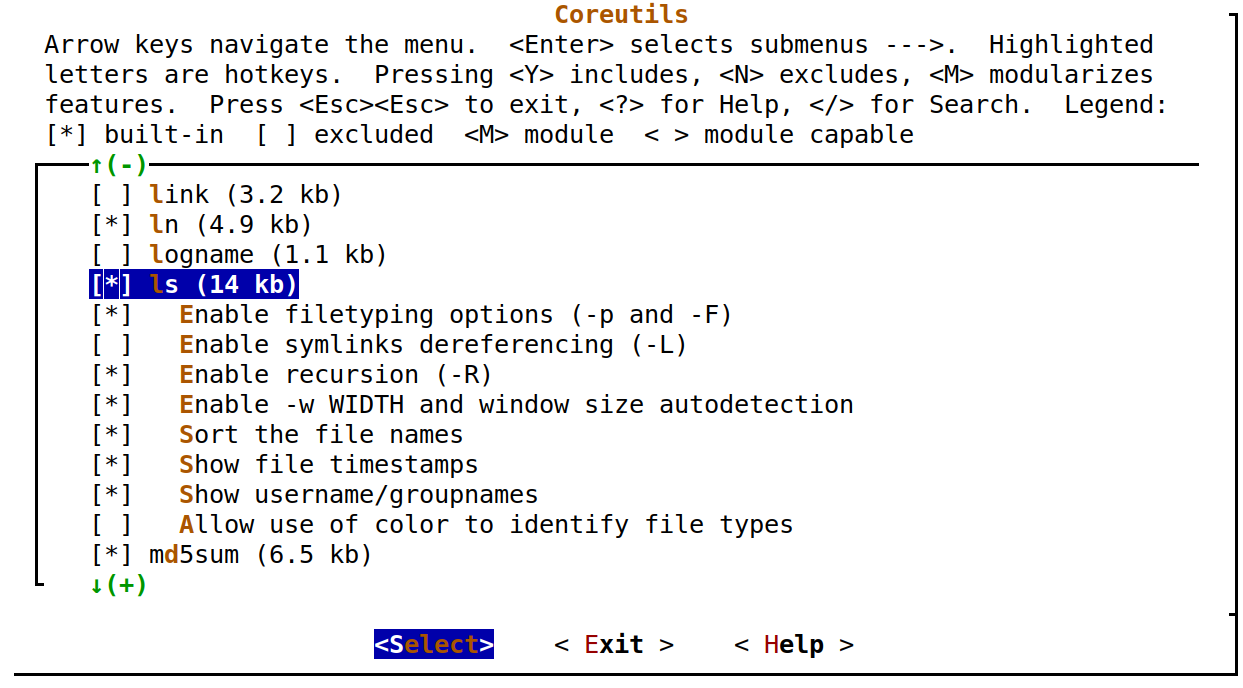
\includegraphics[width=\textwidth]{slides/sysdev-busybox/menuconfig-screenshot.png}
  \end{columns}
\end{frame}

\begin{frame}
  \frametitle{Compiling BusyBox}
  \begin{itemize}
  \item Set the cross-compiler prefix in the configuration interface: \\
    \code{Settings ->  Build Options ->  Cross Compiler
      prefix}\\
    Example: \code{arm-linux-}
  \item Set the installation directory in the configuration interface: \\
    \code{Settings ->  Installation Options}
    \code{  ->  Destination path for 'make install'}
  \item Add the cross-compiler path to the PATH environment variable:\\
    \code{export PATH=$HOME/x-tools/arm-unknown-linux-uclibcgnueabi/bin:$PATH}
  \item Compile BusyBox:\\
    \code{make}
  \item Install it (this creates a UNIX directory structure with symbolic
    links to the \code{busybox} executable):\\
    \code{make install}
  \end{itemize}
\end{frame}

\begin{frame}
  \frametitle{Applet highlight: BusyBox init}
  \begin{itemize}
  \item BusyBox provides an implementation of an \code{init} program
  \item Simpler than the init implementation found on desktop/server
    systems ({\em SysV init} or {\em systemd})
  \item A single configuration file: \code{/etc/inittab}
    \begin{itemize}
    \item Each line has the form \code{<id>::<action>:<process>}
    \end{itemize}
  \item Allows to start system services at startup, to control system
        shutdown, and to make sure that certain services are always
        running on the system.
  \item See \projfile{busybox}{examples/inittab} in BusyBox for details on the
    configuration
  \end{itemize}
\end{frame}

\begin{frame}
  \frametitle{Applet highlight - BusyBox vi}
  \begin{columns}
    \column{0.6\textwidth}
      \begin{itemize}
      \item If you are using BusyBox, adding \code{vi} support only adds
        about 20K
      \item You can select which exact features to compile in.
      \item Users hardly realize that they are using a lightweight \code{vi}
        version!
      \item Tip: you can learn \code{vi} on the desktop, by running the \code{vimtutor}
        command.
      \end{itemize}
    \column{0.4\textwidth}
      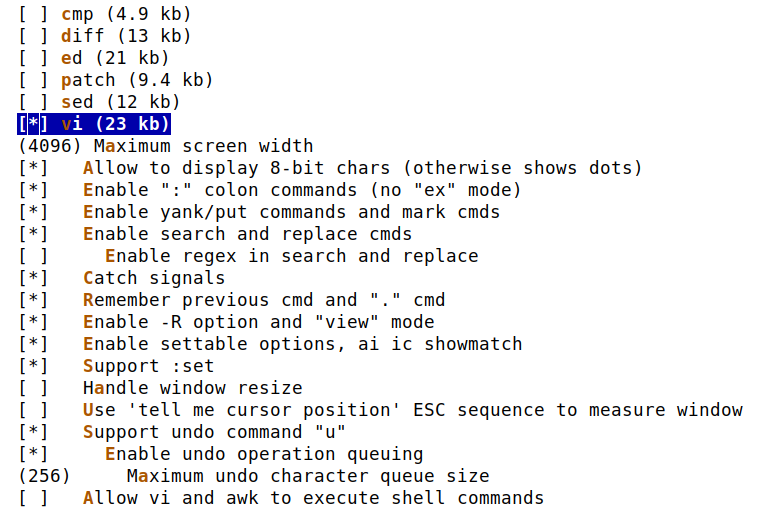
\includegraphics[width=\textwidth]{slides/sysdev-busybox/busybox-vi-configuration.png}
  \end{columns}
\end{frame}

% \setuplabframe
% {Tiny root filesystem built from scratch with BusyBox}
% {
%   \begin{itemize}
%   \item Setting up a kernel to boot your system on a workstation
%     directory exported by NFS
%   \item Passing kernel command line parameters to boot on NFS
%   \item Creating the full root filesystem from scratch.
%     Populating it with BusyBox based utilities.
%   \item System startup using BusyBox \code{init}
%   \item Using the BusyBox HTTP server.
%   \item Controlling the target from a web browser on the PC host.
%   \item Setting up shared libraries on the target and compiling
%     a sample executable.
%   \end{itemize}
% }
